\documentclass[conference]{IEEEtran}
\usepackage{cite}
\usepackage{amsmath,amssymb,amsfonts}
\usepackage{graphicx}
\usepackage{balance}
\usepackage{textcomp}
\usepackage{xcolor}
\usepackage[T1]{fontenc}
\usepackage[utf8]{inputenc}
\usepackage{newunicodechar,booktabs,tabularx,array,enumitem,url}
\newunicodechar{×}{\ensuremath{\times}}
\newunicodechar{→}{\ensuremath{\rightarrow}}
\newunicodechar{−}{\ensuremath{-}}
\newunicodechar{÷}{\ensuremath{\div}}
\newunicodechar{±}{\ensuremath{\pm}}
\newunicodechar{≥}{\ensuremath{\geq}}
\newunicodechar{≤}{\ensuremath{\leq}}
\newunicodechar{ε}{\ensuremath{\varepsilon}}
\newunicodechar{…}{\ldots}
\newunicodechar{§}{\S}
\setcounter{topnumber}{3}
\setcounter{totalnumber}{5}
\renewcommand{\topfraction}{0.9}
\renewcommand{\textfraction}{0.07}
\renewcommand{\floatpagefraction}{0.7}
\setlist{itemsep=0pt,topsep=2pt,parsep=0pt,leftmargin=*}
\newcolumntype{L}{>{\raggedright\arraybackslash}X}
\renewcommand{\arraystretch}{1.15}
\setlength{\emergencystretch}{3em}
\hbadness=10000 \hfuzz=3pt \vfuzz=2pt
\urlstyle{same}
\hyphenation{Mickens}
\raggedbottom
\begin{document}
\title{When Does Adapting Concurrency and Range Size Help? Adaptive Downloading versus aria2 and Fixed Settings under Non-Optimal Conditions}
\author{\IEEEauthorblockN{Sourajyoti Basak}
\IEEEauthorblockA{\textit{Vellore Institute of Technology}\\
Vellore, Tamil Nadu, India - 632014\\
sourajyoti.basak2024@vitstudent.ac.in}
\and
\IEEEauthorblockN{Shwetank Shrijan}
\IEEEauthorblockA{\textit{Vellore Institute of Technology}\\
Vellore, Tamil Nadu, India - 632014\\
shwetank.shrijan2024@vitstudent.ac.in}
\and
\IEEEauthorblockN{Ayush Konar}
\IEEEauthorblockA{\textit{Vellore Institute of Technology}\\
Vellore, Tamil Nadu, India - 632014\\
ayush.konar2024@vitstudent.ac.in}}
\maketitle

\begin{abstract}We asked when adapting the number of connections (N) and the range size (S) during an HTTP range download beats aria2 and the best fixed setting of the same engine, and whether any gain comes from the controller or from the file split. On one workload and the original engine, a fixed 16-connection, 4 MiB-range run finished in 20.12 s against 53.56 s for aria2 (30/30 paired runs, time ratio 0.3756, or 62.4 \% less time). Most of that gap traces to range size and request start times: forcing our engine to use 32 MiB ranges moves the ratio to 0.862. On five replayed cellular traces, a counterfactual oracle found almost no headroom for switching N (mean 0.41 \%, against a predeclared 10 \% bar). We then built a server whose per-request rate falls with concurrency. There a one-threshold drop rule beat the best of three fixed settings by 23.4 \%, but aria2 was still faster. An ablation of 230 runs traced aria2's lead to missing straggler splitting and, we infer, a 30 s request timeout; with both fixed, the best fixed setting beat the controller (1.071 [1.054, 1.085]). Agents retrained for the capped server beat a same-size 1 MiB baseline (0.907 [0.893, 0.921]) but were 1.298 against 16 × 32 MiB and 1.310 against aria2. Adaptive arms beat aria2 only while the server rate was rising. Apart from a small live pilot with one client and four public mirrors, we tested none of this on a production network.\end{abstract}
\begin{IEEEkeywords}HTTP range requests, segmented downloading, concurrency adaptation, aria2, reinforcement learning, network measurement\end{IEEEkeywords}

\section*{I. Introduction}

aria2, axel and lftp choose how many connections to run (N) and how large each range should be (S) before the first byte arrives, then keep those settings. That choice is made for a path that may not hold: a server can slow down and recover, begin to penalise concurrent requests, or a mobile link can swing by an order of magnitude. A controller could move N and S in response. In our experiments, on one machine and our own servers, the engine and the split accounted for more of the observed gap than any controller did.


We ask when adapting N and S can help at all. We compare the main adaptive arms with aria2 and, more importantly, with the best fixed setting of our own engine. Most of the work is infrastructure. The downloader is a Go program in which a policy returns one action at a time, and a checker recomputes all 233 quoted numbers from raw run files. We then ran a direct comparison with aria2, replayed five cellular traces, built a cap, and trained a set of learned policies. Of these, the aria2 comparison matters most, since we characterised the workload first and did not tailor it to adaptation.


\section*{II. Related work}

Balaprakash et al. \cite{balaprakash2016direct} treat the number of parallel streams as an online optimisation problem. Falcon \cite{arifuzzaman2021online,arifuzzaman2023falcon} tunes concurrency through a utility function, and FastBioDL \cite{swargo2025fastbiodl} applies gradient descent to genomic downloads. They tune concurrency or stream counts against observed throughput; Falcon's utility also penalises packet loss and extra concurrency. We ask a prior question: on a server whose mechanism we control, is there any optimum a causal controller could follow?


MDTP \cite{abdollah2025mdtp} sizes chunks across replica servers and uses aria2 \cite{aria2manual} as a baseline; HTTP ranges are defined in RFC 9110 \cite{rfc9110}. We stay with a single source. BOLA \cite{spiteri2020bola} chooses video bitrates without prediction, and DeLoad \cite{liu2025deload} learns download-task sizes for video. Our setting is a single-source range download, where N and S are the only dials.


In the papers we read in full (MDTP, Balaprakash et al., the journal version of Falcon and FastBioDL) we found no swept best-fixed ceiling used as the baseline for a controller, and no ablation that separates engine effects from control. MDTP tunes the chunk size of its own static variant and compares against an untuned aria2. Falcon compares against Globus, HARP, a fixed 32 and a hand-picked 4, and reports cases where it lost; Balaprakash et al. compare against Globus defaults and use a concurrency sweep only as motivation. We did not find a study that sweeps the best fixed setting of one engine and compares it with stock tools. We know BOLA, DeLoad and the earlier Falcon paper from their abstracts only. We propose no new tuning algorithm.


\section*{III. System and experimental platform}

\textbf{Evidence:} Every number is recomputed from raw runs by \texttt{tools/\allowbreak{}claims\_check.py}; block intervals quantify emulator noise, not population variability.




The downloader is a Go program with one decision point. A policy sees the current state and returns a single action: raise or lower N, raise or lower S, or do nothing. A serialized runner applies that action before the next range is allocated. We keep one decision in flight. Fixed rules, threshold rules, LinUCB and Double DQN all use the same path, so the downloader code is identical for every policy (Fig.~\ref{fig:architecture}).


\begin{figure}[!t]\centering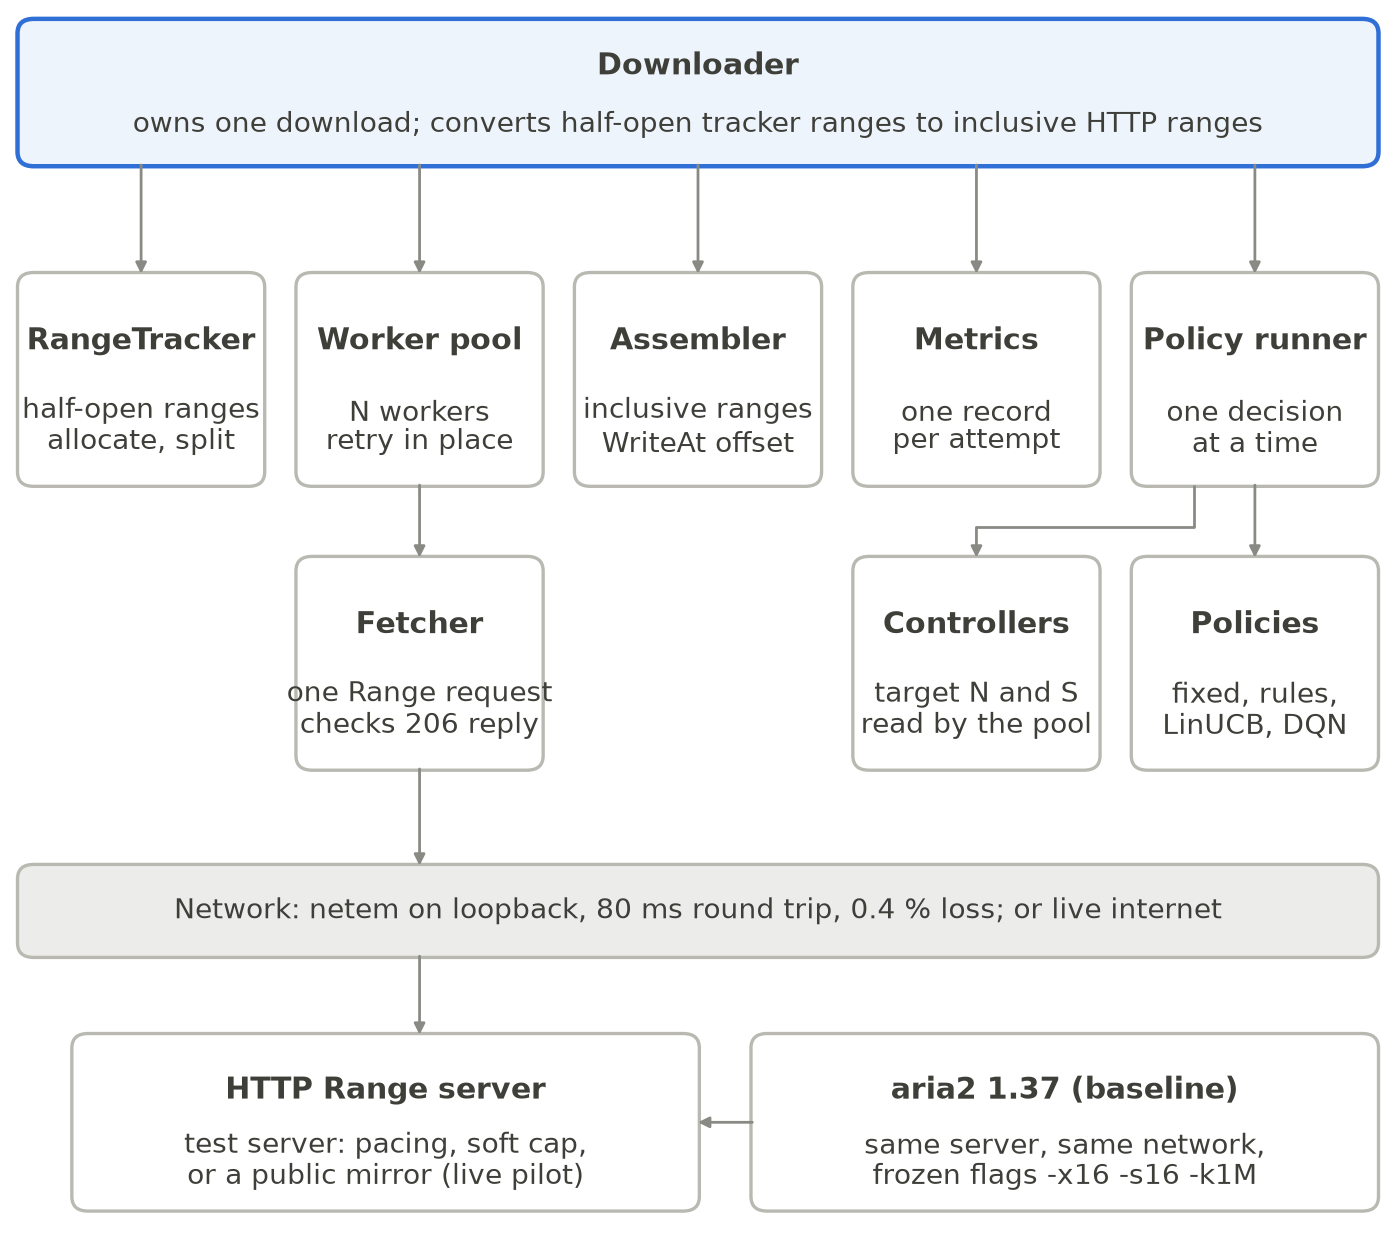
\includegraphics[width=\columnwidth]{figures/architecture.png}\caption{System architecture. One Downloader coordinates five parts; only the Fetcher talks to the network, and policies act only through the controllers. A policy returns one action, the serialized runner applies it, and SHA-256 checks every output file.}\label{fig:architecture}\end{figure}

The range tracker owns allocation and works in half-open intervals. The fetcher turns each one into an inclusive HTTP Range header, and the assembler writes completed ranges to the output file. A range that is already in flight is never resized or cancelled. Changes to N or S affect future allocations only. Every output is checked with SHA-256.


The controlled server serves a deterministic logical object. It fixes a response's rate when the request arrives and holds that rate for the response, which makes request-start timing visible. It can also apply wall-clock pacing schedules, inject faults, and enforce a soft concurrency cap at request start, Eq.~(\ref{eq:cap}):


\begin{equation}\label{eq:cap}r_{\mathrm{eff}} = \min\left\{r_0,\ \frac{C}{k\,(1+\gamma\,(k-1))}\right\}, \qquad k \ge 1\end{equation}

Here $r_0$ is the base rate, $k$ counts concurrent requests including the arriving one, and C = 8 MiB/s with $\gamma$ = 0.05. A live-rate mode re-evaluates the rate during a response and serves as a control. The harness drives aria2, axel, lftp, curl and NGINX, and adds tc/netem delay and loss \cite{tcnetem} and Mahimahi trace replay \cite{netravali2015mahimahi}.


Client and server run on one machine over loopback with netem; the server's pacing, not TCP congestion control, is the bottleneck. The client uses HTTP/1.1 with up to 16 connections, and aria2, axel and lftp also open one connection per segment. Runs are paired in blocks: a block is one run of every arm, in randomised order. Ratios are geometric means over blocks, Eq.~(\ref{eq:ratio}), and intervals are 95 \% t-intervals on the log ratio or percentile bootstraps. Screens use 3–5 blocks and are labelled as such. Because the emulated server is nearly deterministic, those intervals describe emulator repeatability rather than variation across networks. We did not correct for multiplicity or run a power analysis.


\begin{equation}\label{eq:ratio}R = \exp\left(\frac{1}{m}\sum_{i=1}^{m}\ln\frac{t_i^{\mathrm{ours}}}{t_i^{\mathrm{aria2}}}\right)\end{equation}

Here $m$ is the number of paired blocks and $t_i$ is a completion time.


\section*{IV. The aria2 gap is mostly the split}

The characterised workload, D2, is a 512 MiB object. The server paces each response at 640 KiB/s, drops to 160 KiB/s at 2 s, and recovers to 2500 KiB/s at 4 s; netem adds 40 ms each way and 0.4 \% loss (80 ms round trip). Both systems download the same object. Ours uses 16 connections and 4 MiB ranges. aria2 1.37 runs with \texttt{--max-connection-per-server=16 --split=16 --min-split-size=1M}. We tried no other aria2 options, so the results are for aria2 as configured.


Thirty fresh pairs gave 20.12 s for ours and 53.56 s for aria2, a geometric time ratio of 0.3756 [0.3726, 0.3787], with 30/30 wins and all outputs content-verified. In wall-clock terms that is 62.4 \% less time, or 2.66× throughput. Neither system changed N or S, so this is a fixed-configuration result. The runs also use the pre-fix engine; on the corrected engine ours stayed faster than aria2 in the no-cap and D2 cases (0.344 and 0.370).


The server sets a response's rate at arrival. aria2 issues 16 requests — one probe and 15 × 32 MiB ranges — all before 2 s. Every one is held at 640 KiB/s and takes about 51 s. Our engine issues 128 × 4 MiB ranges over the same 16 connections. An early range takes about 6 s, so connections free up after the recovery, and 112 of the 128 ranges start after 4 s at 2500 KiB/s. Both use 16 connections; only the split changes when requests start.


When we force our engine to use 32 MiB ranges, the ratio moves from 0.376 to 0.862 [0.834, 0.890], and most of the gap disappears. aria2's own split settings (16, 64 and 256 initial pieces) do not produce finer initial pieces, so 32 MiB is the closest same-granularity control we have. Request-start timing and pacing explain much of the rest, but not all of it: a constant-fast schedule removes most of the 4 MiB vs 32 MiB difference inside our engine, yet we remain faster than aria2 (15.3 s vs 24.8 s).


The same pattern appeared with axel and lftp. In a five-block screen, ours took 0.345–0.375 of axel's and lftp's time on the healthy and slow–dip–fast scenarios. With the cap starting at 8 s (CAP8), all four tools finished at about 53 s. With the cap from the start (CAP0), axel was 2.5 \% faster and lftp 1.7× slower because it never re-splits. Against stock NGINX per-response rate limiting (configurations N1 and N2) we won every pair in two 5-pair screens (0.863 and 0.597); NGINX limits each response independently, not concurrency, so this checks direction only. The delay × loss sweep went our way in 9/9 cells (0.362–0.457). One expectation failed: at the same nominal per-response rate our own server gave 0.998 on its always-slow schedule, so the N1 comparison is also a direction check. The 14 \% gap between the N1 ratio (0.863) and the 0.998 from our own server remains unexplained. Table~\ref{tab:screens} collects the screens; Fig.~\ref{fig:fig1_ours_vs_aria2} shows the paired ratios.


\begin{figure}[!t]\centering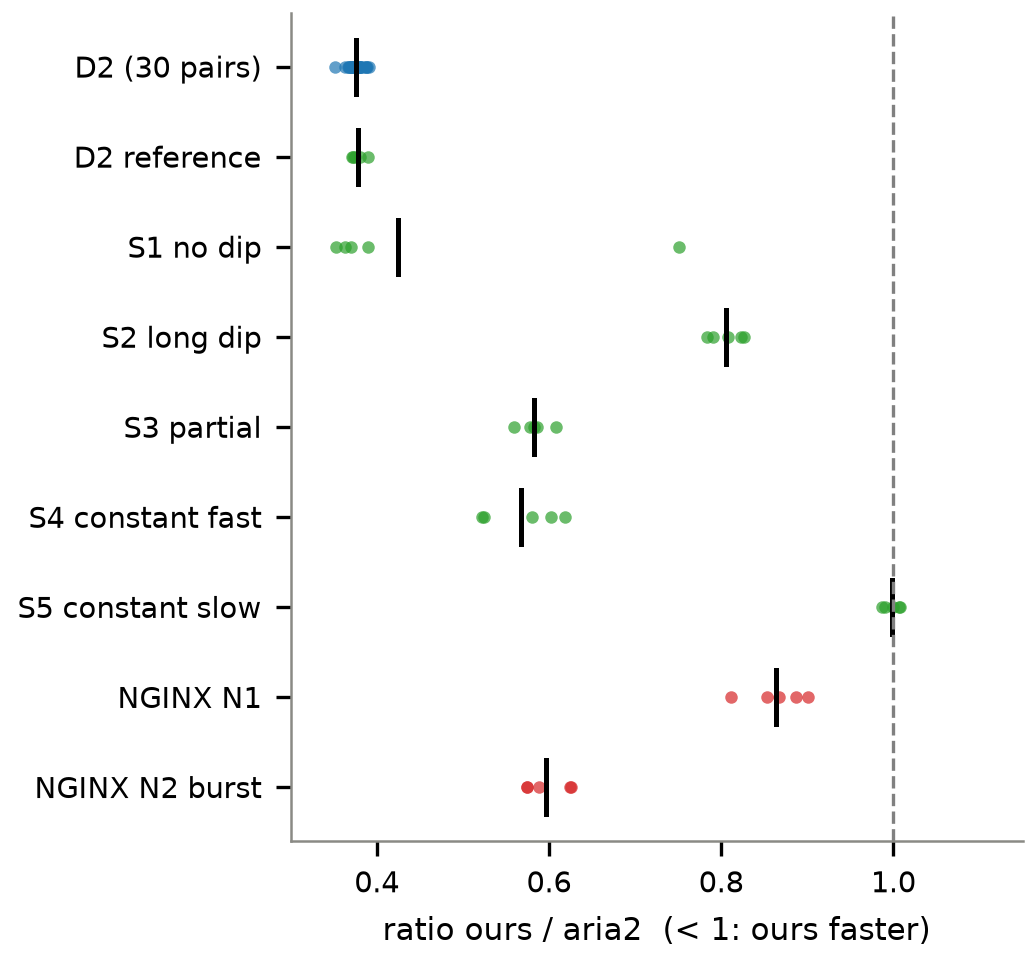
\includegraphics[width=\columnwidth]{figures/fig1_ours_vs_aria2.png}\caption{Paired completion-time ratios ours/aria2 for the frozen D2 benchmark, pacing schedules S1–S5 (no dip, long dip, partial, constant fast, constant slow) and two NGINX configurations (N1, N2). Below 1 means ours was faster; each dot is one block and the tick is the geometric mean. Schedule and NGINX cells are five-pair screens.}\label{fig:fig1_ours_vs_aria2}\end{figure}


\begin{table*}[!t]\centering\footnotesize
\caption{Screening results for the aria2 comparison and other tools. Ratios are ours over the other tool, so below 1 means ours was faster. Except for the 30-pair D2 row, screens have 3–5 pairs and carry no inferential claim.}
\label{tab:screens}
\begin{tabularx}{\textwidth}{@{}>{\hsize=0.9\hsize\raggedright\arraybackslash}X>{\hsize=0.3\hsize\raggedright\arraybackslash}X>{\hsize=1.8\hsize\raggedright\arraybackslash}X@{}}
\toprule
\textbf{Screen} & \textbf{Pairs} & \textbf{Result}\\
\midrule
Frozen D2 benchmark & 30 & 0.376 [0.373, 0.379], 30/30\\
Six pacing schedules & 5 each & 28/30 wins, 0.38–0.81; parity 0.998 on always-slow\\
NGINX rate limit & 5 each & 10/10 wins, 0.863 and 0.597\\
axel and lftp & 5 each & 0.345–0.375 on healthy/D2; CAP0 axel 1.025, lftp 0.597\\
Delay × loss & 3 each & 9/9 cells, 0.362–0.457\\
\bottomrule
\end{tabularx}
\end{table*}


\section*{V. Concurrency headroom on replayed traces}

Five recorded cellular traces (Verizon EVDO/LTE, AT\&T LTE, T-Mobile LTE/UMTS) were replayed through mm-link. Capacity between the 10th and 90th percentile of 1 s bins swings by 6.5–25.3×. Before training a learner, we asked how much of that variation a perfect concurrency switcher could convert into completion time.


For each trace, a fixed-N pilot measured throughput at N = 1, 2, 4, 8 and 16 in every 120 s epoch. The best fixed N is the column with the smallest summed epoch time. The switching oracle solves a dynamic program over epochs: it may stay or move to an adjacent N on the ladder, pays a measured transition cost, and must dwell for one epoch after a change. It sees the measured rate table, not the future of an unknown network. The oracle minimizes the summed epoch times plus transition costs, and headroom is the relative saving over the best fixed N, Eq.~(\ref{eq:oracle}):


\begin{equation}\label{eq:oracle}\begin{aligned} T_{\mathrm{sw}} &= \min_{\{n_t\}} \sum_{t=1}^{T}\left[\tau_t(n_t)+c(n_t,n_{t-1})\right],\\ H &= \frac{T_{\mathrm{fix}}-T_{\mathrm{sw}}}{T_{\mathrm{fix}}}. \end{aligned}\end{equation}

Here $\tau_t(n)$ is the measured time of epoch $t$ at concurrency $n$, $c(n,n')$ is the measured transition cost, and $T_{\mathrm{fix}}$ is the best fixed-N time.


Per-trace headroom was 1.64 \%, 0.019 \%, 0.016 \%, 0.061 \% and 0.294 \%, with a mean of 0.406 \%. The one-sided 95 \% lower bound was −0.26 \% against a predeclared 10 \% bar, so the gate failed. It holds only for 120 s epochs, adjacent moves and a one-epoch dwell, so arbitrary policies are outside its scope. Within that restricted model it is an upper bound; it says nothing about faster switching or about S. On a single shared bottleneck every N slows down together, so the best N barely changes. The traces vary capacity only; we added no delay, loss or server behaviour (Fig.~\ref{fig:fig5_oracle_headroom}).


\begin{figure}[!t]\centering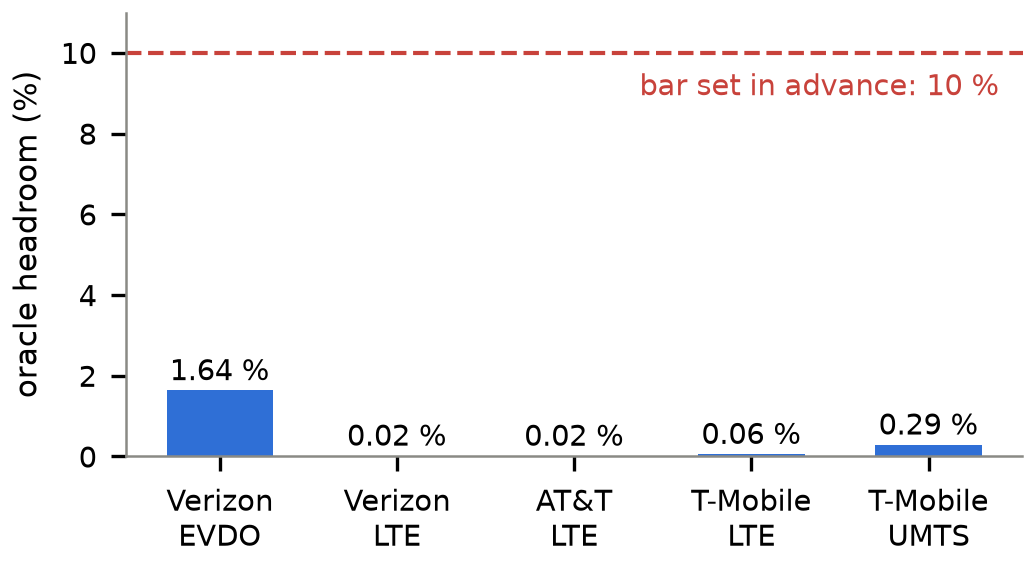
\includegraphics[width=\columnwidth]{../ieee_access/figures/fig5_oracle_headroom.png}\caption{Counterfactual oracle headroom on the five replayed traces. Every trace is far below the 10 \% gate set before the runs.}\label{fig:fig5_oracle_headroom}\end{figure}

Five mechanism screens checked whether any state-dependent optimum existed. They covered static rate plus RTT, a work-conserving queue, correlated loss, failure-based throttling and adaptive-N degradation. The first two left no joint opportunity. Correlated loss made N monotone. Failure-based throttling produced an abort cliff above a threshold. Adaptive-N degradation had an interior optimum on paper, but it did not appear live. Existing adaptive heuristics on D2 adapted and still lost to the fixed optimum; the rule-based joint controller was 2.32× slower than the best fixed setting and won none of 20 blocks. The screens searched a space of server behaviours (72 cap candidates alone), so the cap was found by search. On the original engine it produced such an optimum, but Section VI shows the optimum vanished once the engine was fixed, and the result says nothing about how often one occurs. Only the soft cap in Section VI gave a moving optimum we could see in live runs.


In the pilot, what mattered was opening enough connections. One client on residential broadband downloaded a kernel release from four public mirrors in four time-of-day slots, using eight fixed (N, S) cells plus aria2 and curl. Of 350 runs, 328 were valid (16 were refused by one mirror with HTTP 403, and 6 were lost to an internet drop in a slot that was then re-run in full), giving 16 conditions. A single global 8 × 1 MiB cell was on average 3.7 \% slower than each condition's best (bootstrap 95 \% [1.0, 4.8]); it stayed within 5 \% in 11 of 16 conditions and was at most 15.3 \% slower. The origin mirror needed N ≥ 8, and N = 4 was 1.37–1.71× slower there. The best cell changed across slots on all four servers. In one slot we also reached a second access network by accident; this unplanned, post hoc observation showed 7.2 \% headroom [1.2, 12.2] over four conditions, above the 5 \% line but still inconclusive.


\section*{VI. A cap that penalises concurrency}

We built a server whose per-request rate falls with concurrency and switched the cap on 8 s into the download. On the original engine, the optimum moved from many connections to few in N. The S margin missed its bar, though: five of six predeclared checks passed, the S separation was 3.73 \% [3.09, 4.45] against 5 \%, and three high-N/large-S cells aborted at the 30 s deadline. A one-threshold drop rule watches the windowed median of per-request throughput and switches once to 4 connections and 4 MiB ranges. It finished in 58.7 s against 76.7 s for the best of three fixed settings, a ratio of 0.766 [0.762, 0.769] over 10/10 blocks: 23.4 \% faster. Most of the gain comes from N: N-only took 62.0 s, while S-only took 82.1 s, worse than not switching. aria2 was still faster at 53.6 s (ratio 1.096, 0/10), and Fig.~\ref{fig:fig3_within_download_controller} gives the per-block times.


\begin{figure}[!t]\centering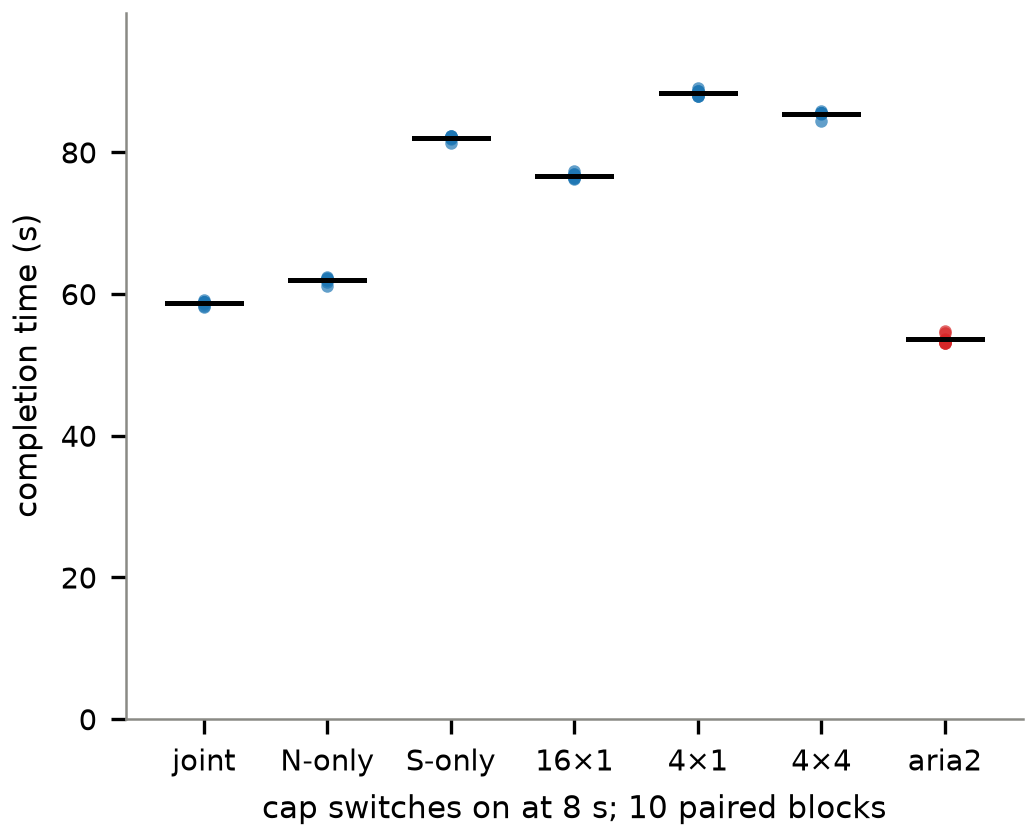
\includegraphics[width=\columnwidth]{figures/fig3_within_download_controller.png}\caption{Cap-from-8-s completion times (10 paired blocks). The causal drop rule beats the best of three fixed settings but is slower than aria2; the S-only ablation is worse than not switching.}\label{fig:fig3_within_download_controller}\end{figure}

We also audited the gap against aria2. Our downloader had a 30 s whole-request deadline that killed a large range which was slow but still progressing, and it never split a slow range; aria2 does both. We made both behaviours opt-in and ran 230 runs over four scenarios × ten shuffled blocks, all valid. Splitting alone cut 40 \% of the capped time (0.599 [0.598, 0.601]) and brought us level with aria2 (68.2 vs 68.5 s, 0.995). Large ranges also required removing the deadline in these runs; we infer the timeout effect but did not isolate it, because 32 MiB with the deadline aborted. With the cap from 8 s, 16 × 32 MiB took 0.711 [0.703, 0.719] of the earlier best fixed time and came within 1.6 \% of aria2 (54.4 vs 53.5 s, 1.016). With both fixes, fixed 16 × 32 MiB matched aria2 and beat the causal controller (1.071 [1.054, 1.085]) and the workload selector on the corrected engine (1.229 [1.223, 1.234]). On that engine the four-connection optimum was gone. Under CAP0 (cap from the start) and CAP8 (cap from 8 s) it was slower than fixed 16 × 32 MiB with splitting. Fig.~\ref{fig:fig4_engine_ablation} shows the part of the earlier adaptive win that came from a weaker engine.


The large-range advantage depends on the server's arrival-rate rule. On a server that re-checks the rate during a response, fixed 16 × 32 MiB slowed from 50.9 s to 67.4 s under the cap.


\subsection*{A. Cross-workload selection}

A separate predeclared family has six workloads, W1–W6: one healthy and five cap, schedule or transition variants. A frozen selector probes at 16 × 1 MiB, classifies after at least 25 s, and applies one predeclared (N, S). In 240 emulated runs on the pre-fix engine (10 blocks per workload, 0 invalid), it came within 0.999 [0.969, 1.029] of the per-workload best fixed setting, but only 0.770 [0.684, 0.859] of the single family-wide best. Block-level intervals treat blocks as independent, so we also computed workload-level intervals over the six workloads: [0.873, 1.143] against the per-workload best and [0.455, 1.304] against the family-wide best. Both include 1, so the point estimates are only descriptive; we have not shown a consistent improvement over one family-wide setting. The frozen model matched 5/6 live optima; W5 mismatched and was not retuned.


\begin{figure}[!t]\centering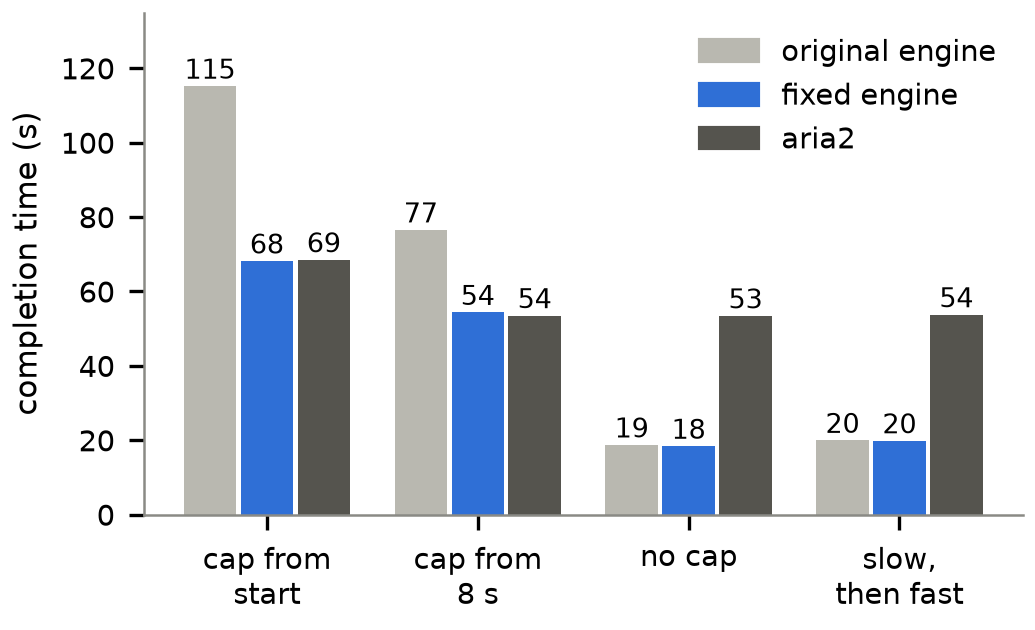
\includegraphics[width=\columnwidth]{../ieee_access/figures/fig4_engine_ablation.png}\caption{Engine ablation: completion time of a fixed configuration on the original engine, on the corrected engine, and of aria2 under four conditions. With both fixes the fixed configuration is level with aria2 or close to it under the cap.}\label{fig:fig4_engine_ablation}\end{figure}

\section*{VII. Learned policies}

All agents use the same serialized runner. LinUCB has five actions (nothing, N ± 1, S ± 4 MiB). The cap-trained DQN has three (nothing, N ± 1) and keeps S at 1 MiB, which isolates the concurrency decision and gives a same-size 1 MiB baseline. The joint DQN adds S ± 4 MiB but moves only 4 MiB per decision, so going from 1 to 33 MiB takes eight decisions.


The early DQN candidates were 1.757×, 2.322× and 1.456× slower than aria2 in their head-to-heads, on 4–16 MiB files and with a ramped start. Those comparisons used the original engine; they test the candidates as built, not whether a learned controller can match aria2.


The retrained agents beat their own 1 MiB baseline but not the best fixed setting or aria2. The cap-trained agent was retrained on a simulator of the capped server and checked blind against live runs: four predictions within 1.4 \%. With the cap from 8 s on a 512 MiB file, it took 0.907 [0.893, 0.921] of the same-size 16 × 1 MiB fixed setting, but stayed slower than 16 × 32 MiB (1.298 [1.274, 1.321]) and aria2 (1.310 [1.287, 1.331]) because it cannot make the large early ranges that keep the pre-cap rate. It won 0 of 3 held-out conditions.


Broader training helped within the training range, barely outside it, and only for the selected seed. Of five seeds, seed 1 was selected on validation, and the other four were mostly at or above the best fixed time. Seed 1's v2 took 0.845 [0.840, 0.850] of fixed 16 × 1 MiB in its home cap, 1.047 without a cap, and won 3 of 4 held-out conditions. A C=8-tuned drop rule was competitive or better in several scenarios. The joint N+S agent took 1.471 [1.405, 1.546] against 16 × 32 MiB, even though a hand-written rule reached 0.352 of the best fixed time in the simulator and live runs matched the simulator's predictions. Table~\ref{tab:agents} summarises the DQN and rule agents.



\begin{table}[!t]\centering\footnotesize
\caption{Learned-policy agents and their main result.}
\label{tab:agents}
\begin{tabularx}{\columnwidth}{@{}>{\hsize=0.8\hsize\raggedright\arraybackslash}X>{\hsize=1.2\hsize\raggedright\arraybackslash}X@{}}
\toprule
\textbf{Agent} & \textbf{Main result}\\
\midrule
Early DQN v2/v5/v6 & 1.757/2.322/1.456× slower than aria2; original engine\\
Cap-trained v1 & 0.907 of same-size fixed; 1.298 vs 16 × 32 MiB; 1.310 vs aria2; 0/3 held out\\
Cap-trained v2 & 0.845 in home cap; 1.047 with no cap; 3/4 held out; 1.2–1.65× slower on mirrors (2 of 3 intervals include parity)\\
Joint N+S & 1.471 vs 16 × 32 MiB; hand rule 0.352 (simulator)\\
Drop rule & competitive; v2 faster in 3, slower in 2, tie in 1 of 6\\
\bottomrule
\end{tabularx}
\end{table}


\subsection*{A. Online tuner}

A FastBioDL-style online tuner was re-implemented as a project policy, not their code. It scores a window by its aggregate throughput $T$ divided by $K^{N}$, where $K$ is a per-connection penalty; we set $K=1$, so the score is simply $T$. It uses 2 s windows, reverses and halves the step after a 5 \% drop, and keeps S at 1 MiB. On the corrected engine it was slower than the better of the two fixed 1 MiB settings in both scenarios: 1.212 [1.180, 1.248] under CAP8 and 1.220 [1.203, 1.232] with no cap. It cut N 2.1 s after the cap, against 1.5 s for the causal rule. Most of its loss comes from the climb: without a cap it needed 8.1 s to go from N = 4 to 16.


\subsection*{B. Synthesis against aria2}

These rows come from different studies, so we do not pool them. A rising server rate was the one condition where adaptive arms beat aria2: 0.36–0.88. A fixed setting of the same engine still did better at 0.344–0.376. Once the rate degraded, the ordering reversed. aria2 beat every adaptive arm (1.096–1.781; the early DQN candidates of Section VII were up to 2.322× slower), and after the engine fix our best fixed 16 × 32 MiB came within 1.6 \%.


These runs use one selected seed, a fixed training envelope, and a 1 MiB action space for the cap agent. On public mirrors, both arms appear to mistake throughput noise for a cap, though we did not test this. v2's point estimate was 1.2–1.65× slower than the better fixed arm and the drop rule's 1.06–1.33× slower, but two of three v2 mirror intervals include parity.


\section*{VIII. Discussion and limitations}

The server models were built and picked from a searched space; none was measured in production. All controlled runs use one machine, loopback plus netem, and one aria2 version, so the 62.4 \% result is explained only in part, by request granularity and start times. We have not shown that it transfers to arbitrary networks. The replay study is weaker in a different way. Its traces vary capacity only, so changing loss or delay during a live download remains untested. The live pilot adds one client on one primary network with four mirrors and two reps per cell, and the learned results use one selected seed with a 1 MiB range for the cap agent; neither establishes a consistent advantage over the best fixed setting or aria2. On the pre-fix engine the W1–W6 selector matched the per-workload best on average (0.999 [0.969, 1.029]) but was not consistently better than one family-wide setting; on the corrected engine it was 1.229 [1.223, 1.234] slower than fixed 16 × 32 MiB (Section VI). We measured completion time, not fairness or the load placed on public mirrors. We did not isolate the 30 s timeout effect, and we did not run a timed open-loop arm, so the drop rule's gain could partly be a schedule effect.


The conclusions come from the measured headroom and from the comparison with the same engine's best fixed setting; aria2 is a second baseline. On this machine and these servers the engine explained more of the difference than the controller. Next we would run a live test with repeated rate cycles and changing loss and delay, then direct range-size actions and deployment-distribution training, reporting every seed.


\section*{IX. Conclusion}

Auditing the engine removed the earlier adaptive win. Missing straggler splitting and, we infer, a 30 s request timeout made aria2 look better than it was under the cap; once both were fixed, a fixed 16 × 32 MiB setting came within 1.6 \% of aria2 and beat the controller on the arrival-rate server. The trace replay found no comparable headroom within its restricted model, and future comparisons should report the engine and the measured opportunity alongside the controller. The 14 \% gap on N1 is still unexplained, and a timed open-loop schedule would separate feedback from timing.


\section*{Availability and AI use}

Raw run files are committed under \texttt{testdata/\allowbreak{}} in the project repository, with SHA-256 checksums in \texttt{SHA256SUMS}. The code, experiment protocols, run manifests and the script that recomputes every quoted number (\texttt{tools/\allowbreak{}claims\_check.py}) are in the project repository: https://github.com/wizard-28/adaptive-downloader


An AI coding assistant (Anthropic Claude, used through Claude Code) helped write the code and analysis scripts, ran experiments and tests, checked results against the raw data, and drafted and edited this text. It generated no data other than by running the specified programs. The authors designed the study, reviewed the results and take responsibility for the content.


\footnotesize
\balance
\bibliographystyle{IEEEtran}
\bibliography{../references}
\end{document}